\subsubsection{Game Design}

\begin{figure}[ht]
    \centering
    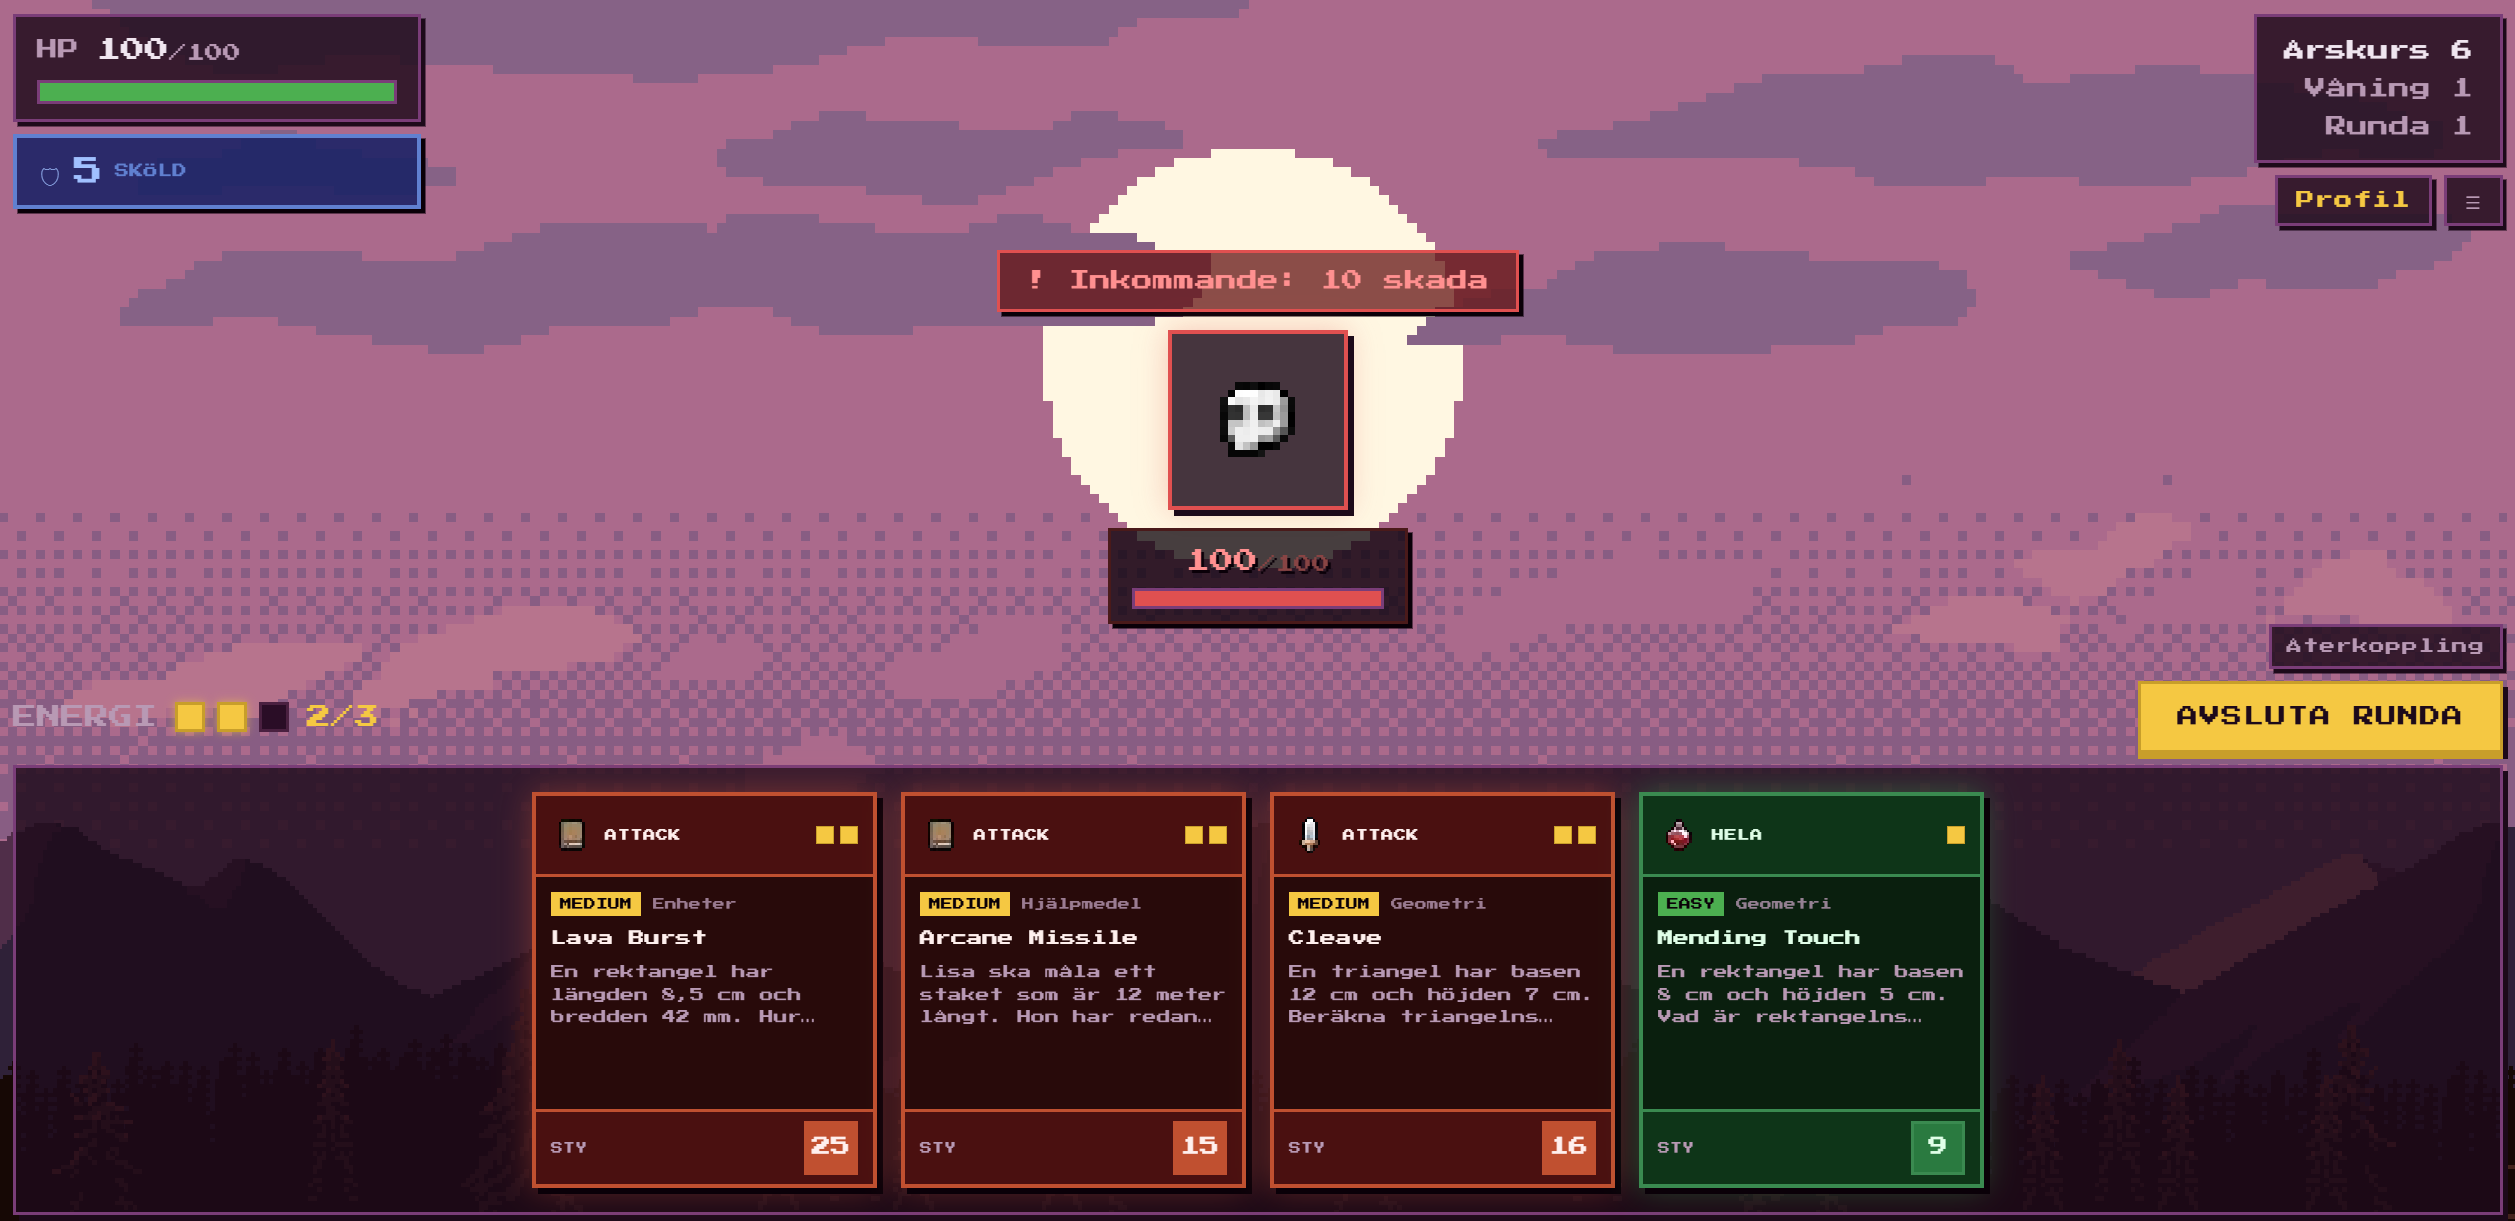
\includegraphics[width=0.8\textwidth]{../images/game_screen.png}
    \caption{The battle screen after a single turn. In the top right we see the players health and active shield. Centered on the screen is the enemy display, showing their health and damage that will be dealt next turn. Cards and their type, strength, energy cost, as well as topic and difficulty of the associated math challenge are displayed in the bottom.}
    \label{fig:game_screen}
\end{figure}

The learner plays a turn-based card combat game inspired by the roguelike deck-building genre. The player is presented with a hand of cards, each displaying its power value and associated challenge difficulty (Figure~\ref{fig:game_screen}). Each card in the player's hand is locked behind a mathematical challenge matched to their current ability level. To play a card, the learner must correctly solve the associated problem. The goal is to defeat an adversary and advance to the next stage, creating a gameplay loop where mathematical reasoning is the core mechanic rather than an interruption.

Cards vary in power, and stronger cards are gated by harder problems. This coupling serves a dual purpose: it motivates learners to attempt more difficult challenges for strategic advantage, and it naturally prevents progress without genuine mathematical engagement. Crucially, incorrect answers carry an in-game consequence in the form of card power reduction, mirroring the stakes of an actual game combat encounter. This mechanic discourages random guessing, ensuring that learners engage thoughtfully with each problem rather than treating the math as a low-cost obstacle to click through~\cite{xu2023exploring}.

\subsubsection{Scaffolding Through the \enquote{MiniGuide} Strategy}

When a learner is stuck on a challenge, they can request help from an in-game agent (Figure~\ref{fig:task_screen}). Rather than providing the answer, the agent follows the \enquote{MiniGuide} strategy: it first diagnoses the learner's current state using the User Model, then retrieves relevant curricular content from a knowledge base via RAG, and finally generates a guiding question designed to nudge the learner toward the solution. This preserves the learner's agency and keeps them actively reasoning.

\begin{figure}[ht]
    \centering
    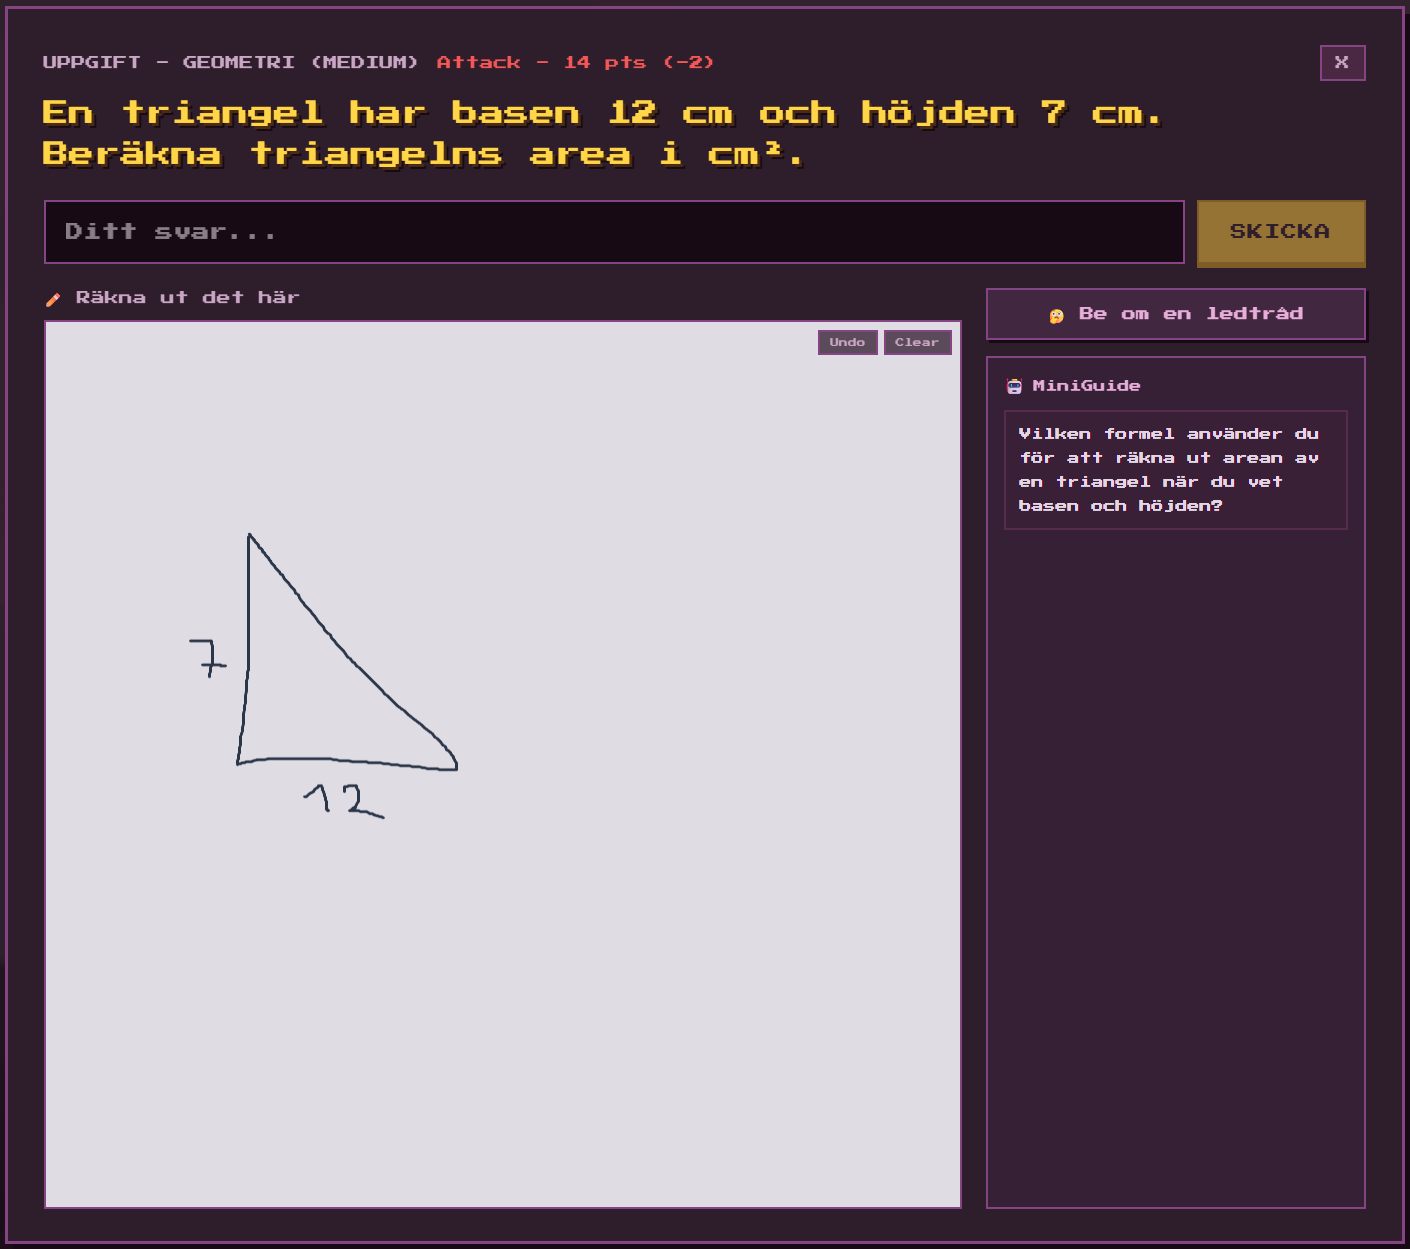
\includegraphics[width=0.8\textwidth]{../images/task_screen.png}
    \caption{The task screen for an easy \enquote{Tid \& Datum} math task, where the answer has been submitted, and the user has requested a hint. The player is presented with the question, a field for entering the answer, a whiteboard for sketching out solutions, and a button for getting a hint with the list of past hints below.}
    \label{fig:task_screen}
\end{figure}

The strict constraint on the generation layer aims to prevent the LLM from producing direct answers. Instead, its output is limited to diagnostic questions, hints, and prompts for reflection — functioning as a peer who helps the learner think, not one who thinks for them.

\subsubsection{Dynamic User Model}

Throughout a learning session, the system builds and refines a User Model that captures the learner's current mastery across mathematical topics, common error patterns, and help-seeking behavior. This model informs both the difficulty of challenges presented and the type of guidance the agent provides. For example, a learner who consistently struggles with fractions will receive challenges and guidance tailored to that gap, while a learner who frequently requests hints without attempting a solution first may receive prompts that encourage independent effort before offering guidance.

In practice, the system tracks correct and incorrect answer attempts and hint requests per difficulty, aggregated by topic. The content of the user model is presented in the user interface as the \enquote{Elevprofil} (Figure~\ref{fig:profile_screen}). When generating new tasks or guiding questions, these metrics are summarized using simple threshold based rules into a learner profile, as shown in Figure ~\ref{fig:user_model_diagram}, identifying strengths, weaknesses, and behavioral patterns, which is then included in the RAG context for subsequent interactions. This means the agent's responses become increasingly personalized over the course of a session, allowing the system to adapt both game difficulty and pedagogical approach to keep the learner within their ZPD.

\begin{figure}[ht]
    \centering
    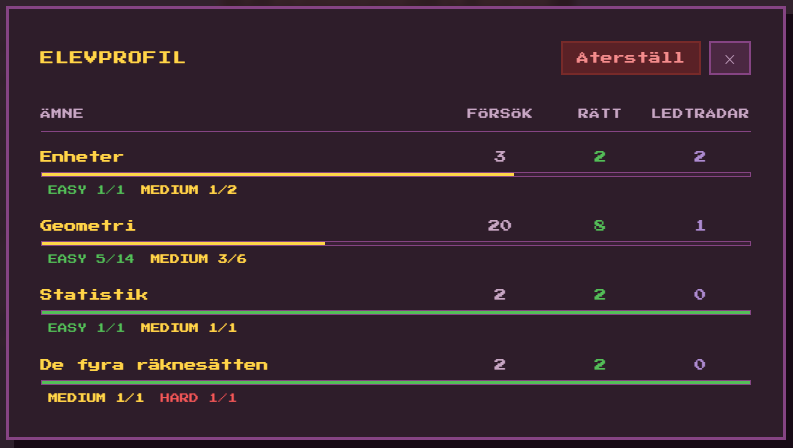
\includegraphics[width=0.8\textwidth]{../images/profile_screen.png}
    \caption{The user model (here called the student profile). The number of answer attempts, correct answers and number of hints received are displayed, grouped by topic.}
    \label{fig:profile_screen}
\end{figure}

\begin{figure}[ht]
    \centering
    \resizebox{0.8\textwidth}{!}{
        \begin{tikzpicture}[
            >={Stealth[length=3mm]},
            box/.style={
                    rectangle, rounded corners=3pt, draw, fill=blue!8,
                    minimum width=3cm, minimum height=1cm,
                    align=center, font=\small
                },
            data/.style={
                    rectangle, rounded corners=3pt, draw, dashed, fill=purple!8,
                    minimum width=3cm, minimum height=1cm,
                    align=center, font=\small\itshape
                },
            llmbox/.style={
                    rectangle, rounded corners=3pt, draw, fill=orange!12,
                    minimum width=3cm, minimum height=1cm,
                    align=center, font=\small
                },
            groupbox/.style={
                    rectangle, rounded corners=5pt, draw=gray!70, dashed,
                    inner sep=12pt
                },
            grouplabel/.style={
                    font=\small\bfseries, text=gray!70
                },
            label/.style={
                    font=\scriptsize, fill=white, inner sep=1pt
                },
            ]

            % Student interactions
            \node[box] (answer) {Answer Attempts};
            \node[box, right=of answer] (topics) {Topic Tags};
            \node[box, right=of topics] (hints) {Hint Requests};

            \node[groupbox, fit=(answer)(topics)(hints)] (metrics) {};
            \node[grouplabel, above=0pt of metrics.north] {Session Metrics};

            % LLM summarization
            \node[llmbox, below=of metrics] (llm) {LLM Summarization};

            % Output
            \node[box, below=of llm] (rag) {RAG Context};

            % Consumers
            \node[box, below left=of rag] (tasks) {Task\\Generation};
            \node[box, below right=of rag] (guidance) {Guidance\\Generation};

            % Arrows
            \draw[->] (metrics) -- (llm);
            \draw[->] (llm) -- (rag);
            \draw[->] (rag) -- (tasks);
            \draw[->] (rag) -- (guidance);

            % Feedback loop
            \draw[->, dashed, gray] (tasks.west) -- ++(-1,0) |-  (answer.west);
            \draw[->, dashed, gray] (guidance.east) -- ++(1,0) |-  (hints.east);

        \end{tikzpicture}
    }

    \caption{User Model creation process.}
    \label{fig:user_model_diagram}
\end{figure}

\subsubsection{Determining the Zone of Proximal Development}

The system approximates each learner's Zone of Proximal Development by classifying problem interactions into three categories based on the level of assistance required.

\begin{description}

    \item [Below:] Problems that the learner solves correctly without requesting any hints, these represent mastered material.\\$\left[Accuracy \geq 70\% \; \& \; hints = 0\right]$

    \item [Above:] Problems where the learner fails to arrive at the correct answer despite available assistance, these are beyond the learner's current reach.\\$\left[Accuracy < 40\% \; \& \; hints \geq 1\right]$

    \item [Within:] Problems that the learner solves correctly after receiving one or more guiding questions from the agent, these are the problems where scaffolding is most effective and where learning is most likely to occur.

\end{description}

This classification, summarized in Figure~\ref{fig:zpd_diagram}, is tracked per topic and accumulated over a session in the form of the user model.

\begin{figure}[ht]
    \centering
    \resizebox{0.8\textwidth}{!}{
        \begin{tikzpicture}[
            >={Stealth[length=3mm]},
            zone/.style={
                    rectangle, rounded corners=5pt, draw,
                    minimum width=9cm, minimum height=1.4cm,
                    align=center, font=\small
                },
            zlabel/.style={
                    font=\small\bfseries, align=right, text width=3cm
                },
            indicator/.style={
                    font=\small, align=left, text width=5.5cm
                },
            ]

            % Zones (stacked bottom to top)
            \node[zone, fill=green!15, draw=green!50!black] (below) {};
            \node[zone, fill=yellow!20, draw=yellow!60!black, above=2pt of below] (within) {};
            \node[zone, fill=red!12, draw=red!50!black, above=2pt of within] (above) {};

            % Zone labels (left side)
            \node[zlabel, left=0.1cm of above] {Above ZPD};
            \node[zlabel, left=0.1cm of within] {Within ZPD};
            \node[zlabel, left=0.1cm of below] {Below ZPD};

            % Indicators (inside zones)
            \node[indicator] at (above.center) {Incorrect despite assistance\\$\rightarrow$ Too difficult, reduce difficulty};
            \node[indicator] at (within.center) {Correct after guiding questions\\$\rightarrow$ Optimal learning zone, maintain};
            \node[indicator] at (below.center) {Correct without hints\\$\rightarrow$ Already mastered, increase difficulty};
        \end{tikzpicture}
    }

    \caption{Classification of problem interactions into ZPD regions.}
    \label{fig:zpd_diagram}
\end{figure}

\subsubsection{Gamification and Motivation}

The game structure is designed to align with Self-Determination Theory~\cite{ryan2000self} by supporting autonomy (choosing which cards to attempt), competence (solving challenges at an appropriate difficulty), and relatedness (interacting with the in-game agent as a supportive peer). Because card power is tied to problem difficulty relative to the learner's level, both high-performing and struggling learners face meaningful challenges — avoiding boredom for advanced students and reducing frustration for those who need more support.

Importantly, progress in the game is closely tied to demonstrated mathematical reasoning, and not surpassable game mechanics or repetition. This transforms the friction of learning into a core part of the game loop rather than an obstacle to it.
